\documentclass[a4paper]{article}
\usepackage{a4wide,amssymb,epsfig,latexsym,multicol,array,hhline,fancyhdr}
\usepackage{float}
\usepackage[utf8]{vietnam}
\usepackage[vietnamese,english]{babel}
\usepackage{amsmath}
\usepackage{lastpage}
\usepackage[lined,boxed,commentsnumbered]{algorithm2e}
\usepackage{enumerate}
\usepackage{color}
\parindent 0pt
\usepackage{graphicx}							% Standard graphics package
\usepackage{array}
\usepackage{tabularx, caption}
\usepackage{multirow}
\usepackage{multicol}
\usepackage{rotating}
\usepackage{graphics}
\usepackage{geometry}
\usepackage{setspace}
\usepackage{epsfig}
\usepackage{tikz}
\usetikzlibrary{arrows,snakes,backgrounds}
\usepackage{hyperref}
\hypersetup{urlcolor=blue,linkcolor=black,citecolor=black,colorlinks=true} 
%\usepackage{pstcol} 								% PSTricks with the standard color package

\newtheorem{theorem}{{\bf Theorem}}
\newtheorem{property}{{\bf Property}}
\newtheorem{proposition}{{\bf Proposition}}
\newtheorem{corollary}[proposition]{{\bf Corollary}}
\newtheorem{lemma}[proposition]{{\bf Lemma}}

\AtBeginDocument{\renewcommand*\contentsname{Contents}}
\AtBeginDocument{\renewcommand*\refname{References}}
%\usepackage{fancyhdr}
\setlength{\headheight}{40pt}
\pagestyle{fancy}
\fancyhead{} % clear all header fields
\fancyhead[L]{
 \begin{tabular}{rl}
    \begin{picture}(25,15)(0,0)
    \put(0,-8){
\includegraphics[width=8mm, height=8mm]{graphics/hcmut.png}}
    %\put(0,-8){\epsfig{width=10mm,figure=hcmut.eps}}
   \end{picture}&
	%
\includegraphics[width=8mm, height=8mm]{hcmut.png} & %
	\begin{tabular}{l}
		\textbf{\bf \ttfamily University of Technology, Ho Chi Minh City}\\
		\textbf{\bf \ttfamily Faculty of Computer Science and Engineering}
	\end{tabular} 	
 \end{tabular}
}
\fancyhead[R]{
	\begin{tabular}{l}
		\tiny \bf \\
		\tiny \bf 
	\end{tabular}  }
\fancyfoot{} % clear all footer fields
\fancyfoot[L]{\scriptsize \ttfamily Assignment for Computer Architecture - Academic year 2023 - 2024}
\fancyfoot[R]{\scriptsize \ttfamily Page {\thepage}/\pageref{LastPage}}
\renewcommand{\headrulewidth}{0.3pt}
\renewcommand{\footrulewidth}{0.3pt}


%%%
\setcounter{secnumdepth}{4}
\setcounter{tocdepth}{3}
\makeatletter
\newcounter {subsubsubsection}[subsubsection]
\renewcommand\thesubsubsubsection{\thesubsubsection .\@alph\c@subsubsubsection}
\newcommand\subsubsubsection{\@startsection{subsubsubsection}{4}{\z@}%
                                     {-3.25ex\@plus -1ex \@minus -.2ex}%
                                     {1.5ex \@plus .2ex}%
                                     {\normalfont\normalsize\bfseries}}
\newcommand*\l@subsubsubsection{\@dottedtocline{3}{10.0em}{4.1em}}
\newcommand*{\subsubsubsectionmark}[1]{}
\makeatother


\begin{document}

\begin{titlepage}
\begin{center}
VIETNAM NATIONAL UNIVERSITY, HO CHI MINH CITY \\
UNIVERSITY OF TECHNOLOGY \\
FACULTY OF COMPUTER SCIENCE AND ENGINEERING
\end{center}

\vspace{1cm}

\begin{figure}[h!]
\begin{center}

\includegraphics[width=3cm]{graphics/hcmut.png}
\end{center}
\end{figure}

\vspace{1cm}


\begin{center}
\begin{tabular}{c}
\multicolumn{1}{l}{\textbf{{\Large COMPUTER ARCHITECTURE (CO2007)}}}\\
~~\\
\hline
\\
\multicolumn{1}{l}{\textbf{{Assignment (Semester: 231)}}}\\
\\
\textbf{{\Huge BATTLESHIP}}\\

\multicolumn{1}{l}{\textbf{{}}}\\
\\
\hline
\end{tabular}
\end{center}

\vspace{2cm}

\begin{table}[h]
	\begin{tabular}{rrl}
		\hspace{5 cm} & Advisor: & Băng Ngọc Bảo Tâm, CSE-HCMUT\\[6pt]
		& Student: & Trần Đình Đăng Khoa \hspace*{0.05cm} - 2211649. \\
	\end{tabular}
\end{table}

\vspace*{1cm}

\begin{center}
{\footnotesize HO CHI MINH CITY, NOVEMBER 2023}
\end{center}
\end{titlepage}

\newpage
\tableofcontents

%%%%%%%%%%%%%%%%%%%%%%%%%%%%%%%%%
\newpage
\section{Introduction}
\qquad Battleship (also known as Battleships or Sea Battle) is a strategy type guessing game for two players. It is played on ruled grids (paper or board) on which each player's fleet of warships are marked. The locations of the fleets are concealed from the other player. Players alternate turns calling "shots" at the other player's ships, and the objective of the game is to destroy the opposing player's fleet. \\[6pt]

\begin{figure}[H]
    \centering
    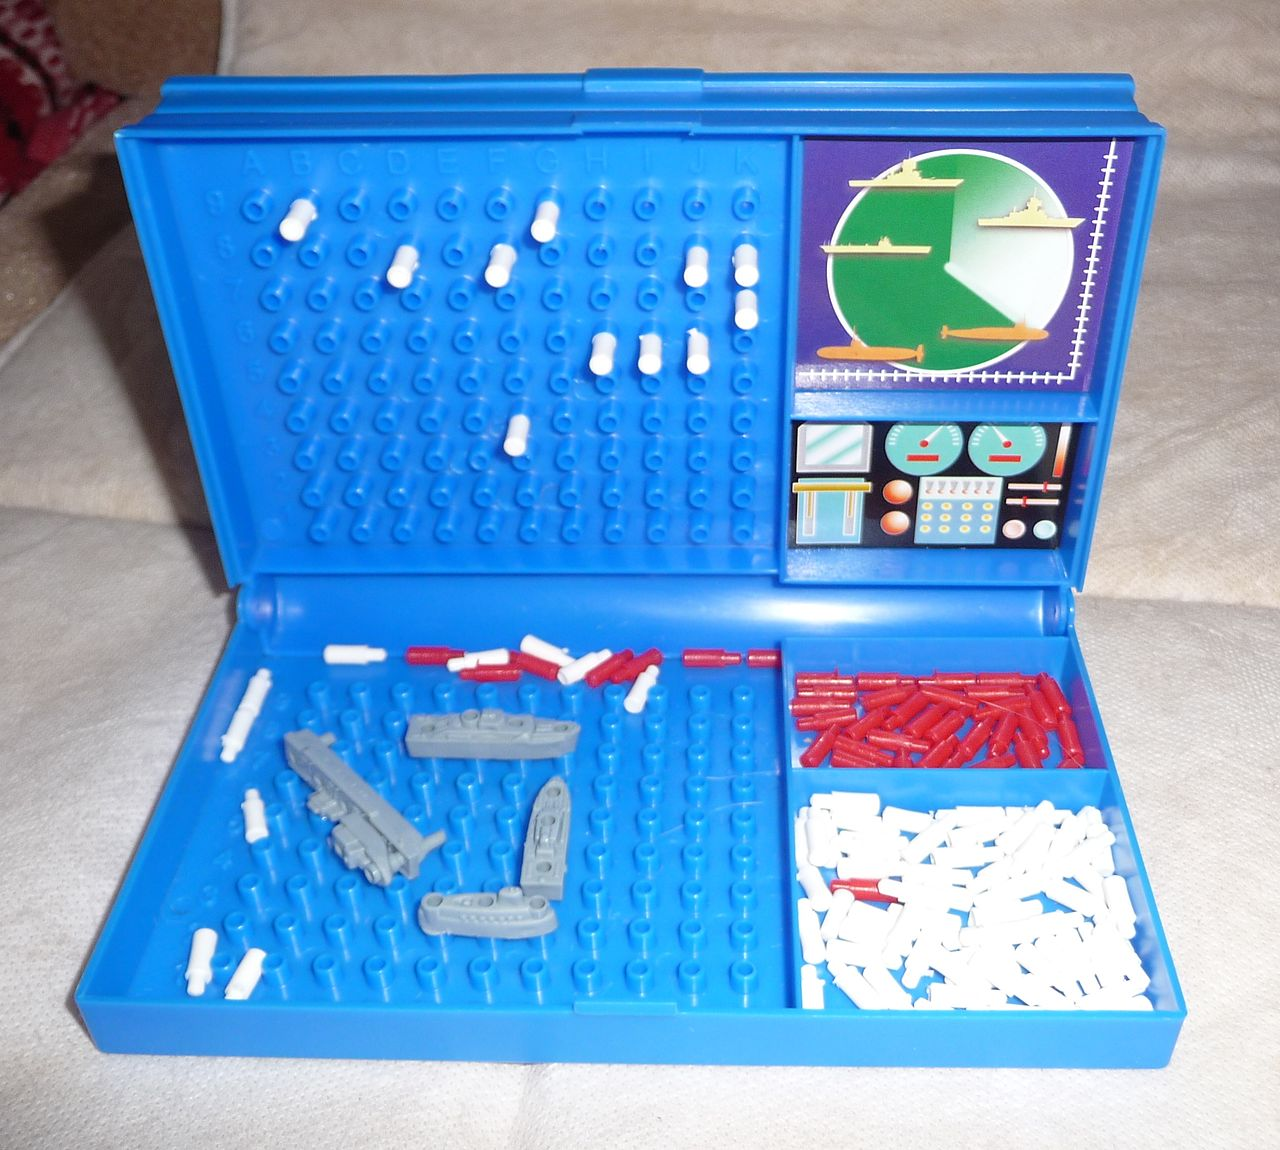
\includegraphics[width=12cm]{graphics/battleship.jpg}
    \selectlanguage{english}
    \caption{Example of the classic battleship game}
\end{figure}

\subsection{Description}
\qquad The game is played on four grids, two for each player. The grids are typically square - usually 10$\times$10 - and the individual squares in the grid are identified by letter and number. On one grid the player arranges ships and records the shots by the opponent. On the other grid, the player records their own shots.\\

\qquad Before play begins, each player secretly arranges their ships on their primary grid. Each ship occupies a number of consecutive squares on the grid, arranged either horizontally or vertically. The number of squares for each ship is determined by the type of ship. The ships cannot overlap (i.e., only one ship can occupy any given square in the grid). The types and numbers of ships allowed are the same for each player. These may vary depending on the rules. The ships should be hidden from players sight and it's not allowed to see each other's pieces. The game is a discovery game which players need to discover their opponents ship positions.\\

\qquad After the ships have been positioned, the game proceeds in a series of rounds. In each round, each player takes a turn to announce a target square in the opponent's grid which is to be shot at. The opponent announces whether or not the square is occupied by a ship. If it is a "hit", the player who is hit marks this on their own or "ocean" grid (with a red peg in the pegboard version), and announces what ship was hit. The attacking player marks the hit or miss on their own "tracking" or "target" grid with a pencil marking in the paper version of the game, or the appropriate color peg in the pegboard version (red for "hit", white for "miss"), in order to build up a picture of the opponent's fleet.\\

\qquad If all of a player's ships have been sunk, the game is over and their opponent wins.
%%%%%%%%%%%%%%%%%%%%%%%%%%%%%%%%%
\section{MIPS Assembly Implementation}
\subsection{Introduction}
\qquad In this project, we aim to emulate the Battleship game using the \textit{MIPS} assembly language. Due to resource constraints and to keep things simple, we will work with a smaller grid size which is \textbf{7$\times$7} \\

\qquad A ship location is indicated by the
coordinates of the bow and the stern of the ship (row$_{\text{bow}}$, column$_{\text{bow}}$, row$_{\text{stern}}$, column$_{\text{stern}}$). 

\begin{figure}[H]
    \centering
    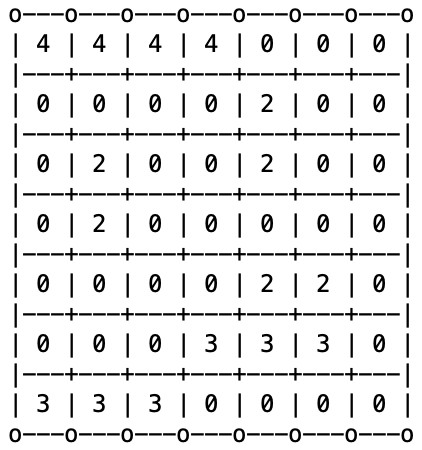
\includegraphics[width=10cm]{graphics/intromap.jpg}
    \selectlanguage{english}
    \caption{Map}
\end{figure}

In the above figure, the coordinates of the \textbf{4$\times$1} ship is \texttt{0 0 0 3}; the green \textbf{3$\times$1} ships are \texttt{5 3 5 5} and \texttt{6 0 6 2}; the \textbf{2$\times$1} ships are \texttt{1 4 2 4},   \texttt{2 1 3 1}, and \texttt{4 4 4 5}. \\

\qquad The initial phase involves players arranging their ship positions. The program prompts players to input ship locations on a map where each cell holds either "the ship's size" or "0", indicating an empty/unoccupied space. Specifically, a cell contains the ship's size if occupied, and 0 if empty. During the setup phase, players must precisely position a predefined number of ships, each of the same size. In detail, each player will have 3 \textbf{2$\times$1} ships, 2 \textbf{3$\times$1} ships, and 1 \textbf{4$\times$1} ship. Note that ships can not overlap with each other.

\subsection{Overall Structure}
\begin{enumerate}
    \item \textbf{Data Section (.data):} \\
    The data section serves as the preamble to the program, laying the foundation for essential constants, character values, and game-related data. This section is crucial for establishing the groundwork necessary for the subsequent execution of the game.
        \begin{itemize}
            \item Constants: \\
            Various system calls are defined to facilitate operations such as \textit{printing} integers, strings, \textit{reading} integers, strings, and exiting. Additionally, character values are assigned to digits, letters, and spaces, enhancing the readability and manageability of the code.
            \item Game-related Constants: \\
            This subsection introduces constants that play a pivotal role in the game's mechanics. Values such as \textit{player turns}, the \textit{number of ships}, the \textit{number of cells}, and \textit{input lengths} are defined to ensure consistency and facilitate modifiability.
            \item Data and Variables: \\
            \textit{Arrays} for player A and player B maps are initialized, providing a structured representation of the game state. Strings containing the \textit{game title}, \textit{rules}, \textit{prompts}, and \textit{messages} are declared, contributing to a more comprehensible and user-friendly gaming experience.\\
            Numerous variables are introduced to store critical information, including the \textit{grid size}, \textit{ship coordinates}, and \textit{shot coordinates}. These variables serve as dynamic entities, adapting to the evolving state of the game during execution.
        \end{itemize}

    \item \textbf{Text Section (.text):} \\
    The text section constitutes the heart of the program, containing the main program logic, function calls, and the structural components that orchestrate the flow of the game. It encapsulates the core functionalities responsible for the game's initiation, progression, and termination.
        \begin{itemize}
            \item Main Section:\\
            The main section initializes registers, loads addresses for player maps, and orchestrates the initial setup of the game. It sets the stage for the subsequent execution of the game logic.
            \item Function Calls:\\
            Function calls to \texttt{game\_menu}, \texttt{rules\_screen}, and \texttt{print\_maps} contribute to the modular design of the code. These functions encapsulate specific functionalities, promoting code readability and maintainability.
            \item Game Setup:\\
            The code calls the \texttt{read\_ship} function twice, allowing players to input ship positions for player A and player B. After all the ships have been placed, the \texttt{print\_maps} function is invoked to visualize the current game state.
            \item Game Loop:\\
            The core game loop orchestrates the turn-based shooting mechanism, engaging players in strategic exchanges. Within the loop, players take turns calling the \texttt{read\_shot} function to input coordinates for targeting their opponent's fleet. After each successful shot, the program evaluates the game state to determine if the current player has won. If a player emerges victorious, the game loop concludes, and the \texttt{print\_maps} function is invoked to showcase the final game board with updated ship positions and the winner's triumph. This meticulous updating of the visual representation ensures that players are presented with a clear and conclusive view of the game's outcome.
            \item Exit Section:\\
            The program concludes with an \texttt{exit} section, invoking a system call to terminate the execution gracefully. This ensures proper closure and resource release.
        \end{itemize}

    \item \textbf{Helper Functions} \\
    This subsection delves into the specifics of key functions such as \texttt{read\_ship} and \texttt{read\_shot}. These functions are responsible for \textit{acquiring} user input, \textit{validating} it, and \textit{facilitating the corresponding game actions}.
\end{enumerate}

\subsection{Constants and Definitions}
Explain the purpose of constants defined using .eqv (e.g., system calls, characters, and game-related constants).

\begin{enumerate}
    \item \textbf{System Calls}:
    \begin{itemize}
        \item \texttt{SYS\_PRINT\_INT  \quad}: System call for printing an integer (value: 1).
        \item \texttt{SYS\_PRINT\_STRING}: System call for printing a string (value: 4).
        \item \texttt{SYS\_READ\_INT\qquad}: System call for reading an integer (value: 5).
        \item \texttt{SYS\_READ\_STRING }: System call for reading a string (value: 8).
        \item \texttt{SYS\_EXIT\qquad\qquad}: System call for program exit (value: 10).
        \item \texttt{SYS\_PRINT\_CHAR\quad}: System call for printing a character (value: 11).
        \item \texttt{SYS\_READ\_CHAR   \quad}: System call for reading a character (value: 12).
    \end{itemize}
    \item \textbf{Character Constants:} \\
    Constants representing ASCII values for characters:
    \begin{itemize}
        \item \texttt{char\_0} to \texttt{char\_6}: ASCII values for the characters '0' to '6'.
        \item \texttt{char\_N}: ASCII value for the character 'N'.
        \item \texttt{char\_Q}: ASCII value for the character 'Q'.
        \item \texttt{char\_R}: ASCII value for the character 'R'.
        \item \texttt{char\_Y}: ASCII value for the character 'Y'.
        \item \texttt{char\_n}: ASCII value for the character 'n'.
        \item \texttt{char\_q}: ASCII value for the character 'q'.
        \item \texttt{char\_r}: ASCII value for the character 'r'.
        \item \texttt{char\_y}: ASCII value for the character 'y'.
        \item \texttt{char\_space}: ASCII value for the space character.
    \end{itemize}
    \item \textbf{Player Turn and Game Constants:}
    \begin{itemize}
        \item \texttt{player\_a\_turn}: Value representing Player A's turn (value: 0).
        \item \texttt{player\_b\_turn}: Value representing Player B's turn (value: 1).
        \item \texttt{number\_of\_ships}: Total number of ships each player has (value: 6).
        \item \texttt{number\_of\_cells}: Total number of cells on the grid (value: 49).
        \item \texttt{input\_coordinates\_length\_shot}: Length of input for shot coordinates (value: 4).
        \item \texttt{input\_coordinates\_length\_ship}: Length of input for ship coordinates (value: 8).
    \end{itemize}
    \item \textbf{Player Maps and Grid Size:}
    \begin{itemize}
        \item \texttt{player\_a\_map}: An array representing the map for Player A, initialized with zeros.
        \item \texttt{player\_b\_map}: An array representing the map for Player B, also initialized with zeros.
        \item \texttt{grid\_size}: Word variable storing the size of the grid (value: 7).
    \end{itemize}   
    \item \textbf{Coordinate Spaces:}
    \begin{itemize}
        \item \texttt{ship\_coordinates}: Space reserved for storing ship coordinates during input.
        \item \texttt{shot\_coordinates}: Space reserved for storing shot coordinates during input.
    \end{itemize}
\end{enumerate}

\qquad These directives and data declarations provide symbolic names for system calls, characters, game constants, and storage spaces, making the MIPS assembly code more readable and maintainable. The constants and data structures defined here are used throughout the program to enhance code clarity and facilitate updates.\\

\newpage

\subsection{User Interface}
\begin{enumerate}
    \item \textbf{Game Menu:} \\
    
    The game menu is displayed to the user with ASCII art, creating a visually appealing and thematic presentation. The menu includes a title and options for the user to proceed or start the game. The ASCII art in the title creates a distinctive and engaging visual experience, making the menu more enjoyable for the user. The options to proceed or start the game are presented clearly to guide the user through the initial steps.\\

    \vspace*{2cm}

    \begin{figure}[H]
        \centering
        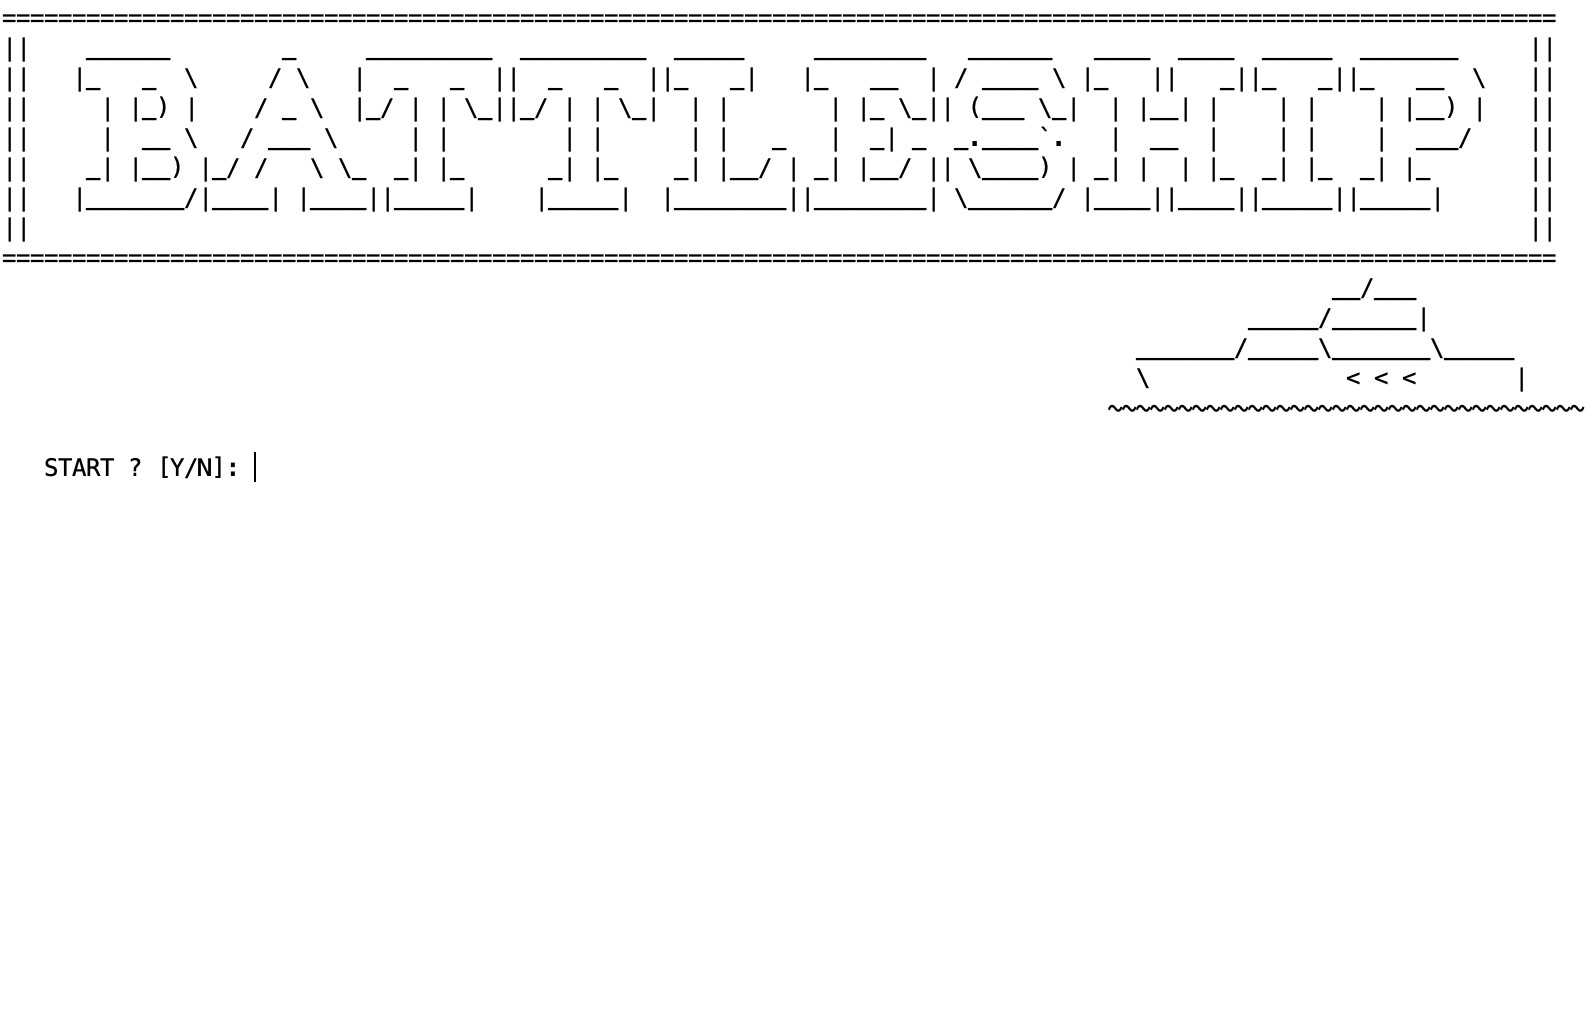
\includegraphics[width=15cm]{graphics/menu.jpg}
        \selectlanguage{english}
        \caption{Game Menu Interface}
    \end{figure}

    \newpage
    \item \textbf{Rules Screen:} \\
    
    The rules screen is presented using ASCII art to provide an immersive and visually interesting display of the game rules. The ASCII art includes a title, setup phase instructions, gameplay details, update board information, winning conditions, and specific rules about ship placement and shooting. Each section is delineated with ASCII borders and design elements, making it easy for the user to navigate and comprehend the rules of the game. The use of ASCII characters enhances the aesthetic appeal of the rules screen, making it both informative and visually engaging for the player.\\

    \begin{figure}[H]
        \centering
        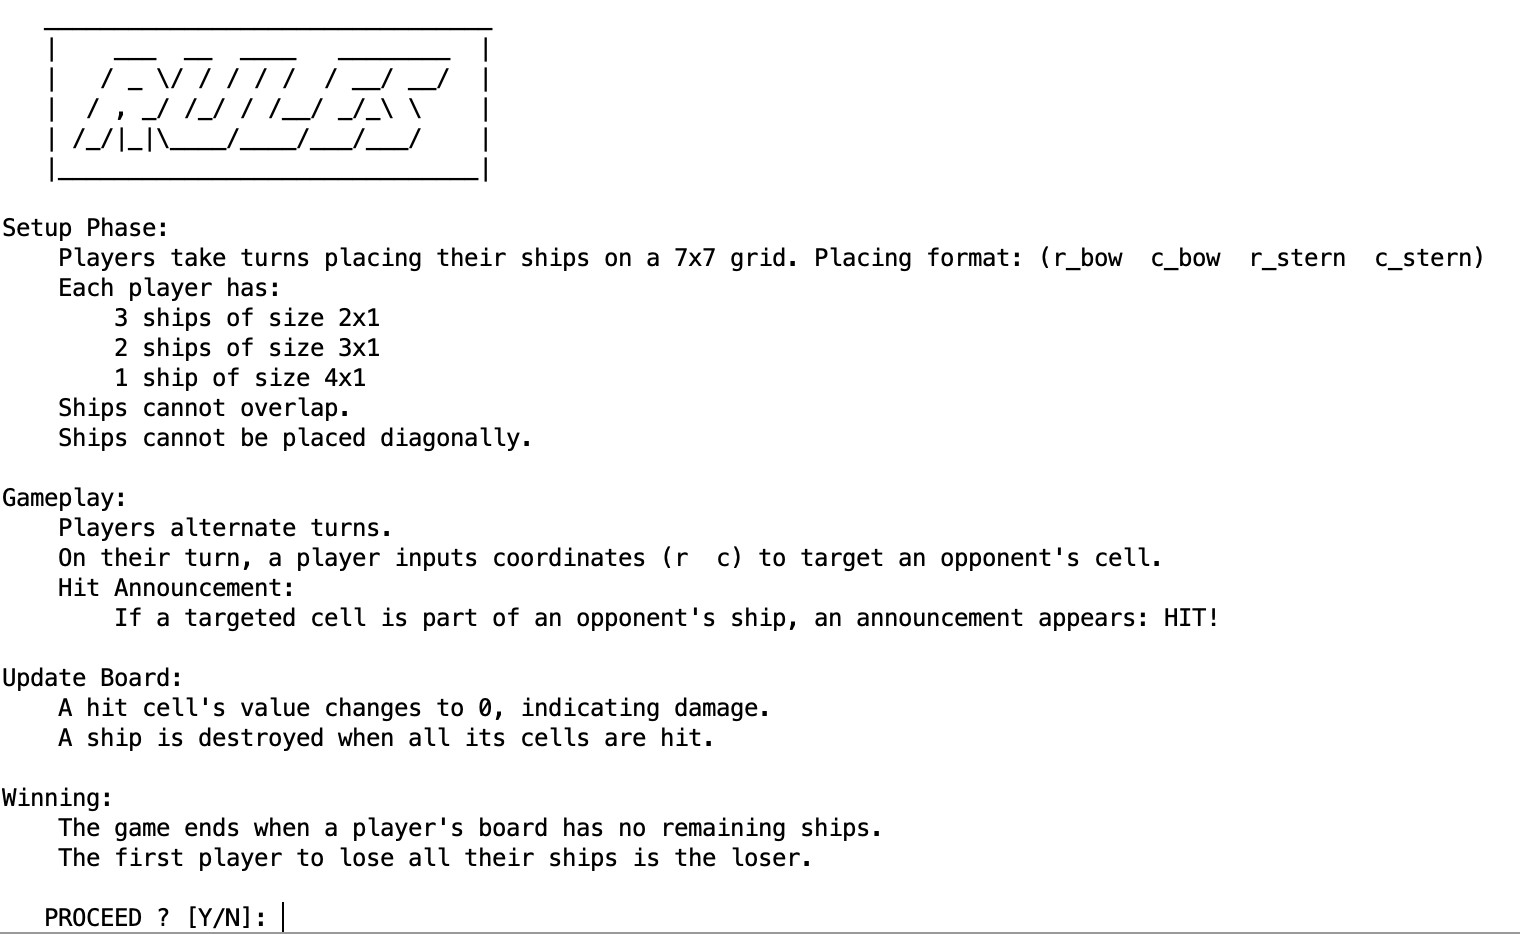
\includegraphics[width=15cm]{graphics/rules.jpg}
        \selectlanguage{english}
        \caption{Rules Screen Interface}
    \end{figure}

    \newpage

    
    \item \textbf{Placing Ships Interface:} \\
    
    \begin{figure}[H]
        \centering
        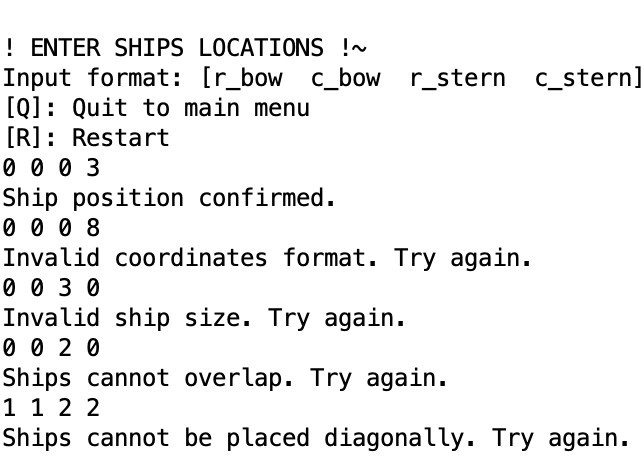
\includegraphics[width=10cm]{graphics/placing.jpg}
        \selectlanguage{english}
        \caption{Placing Ships Interface}
    \end{figure}

    \newpage

    \item \textbf{Shooting and Endgame Interface:} \\
    
    \begin{figure}[H]
        \centering
        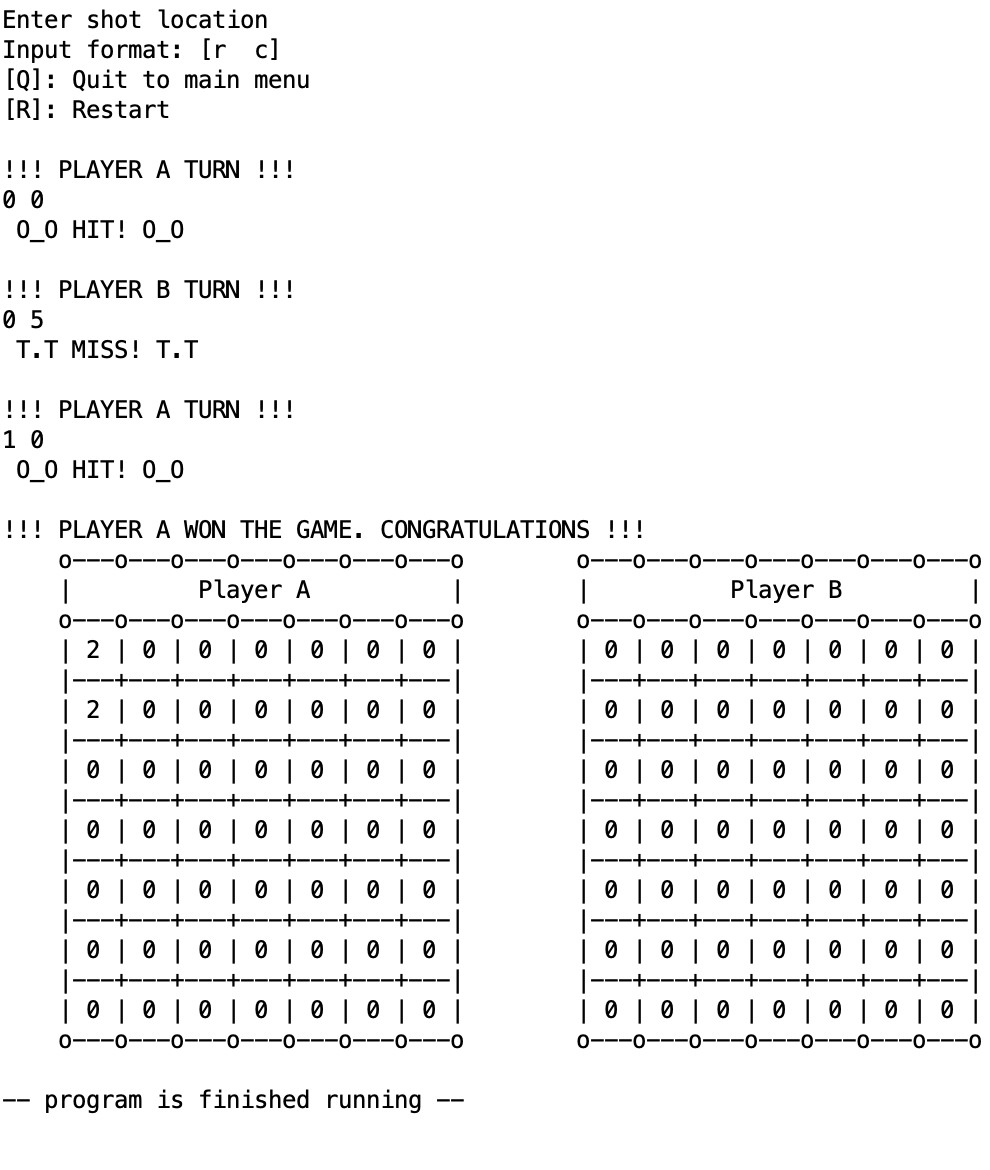
\includegraphics[width=15cm]{graphics/shooting_ending.jpg}
        \selectlanguage{english}
        \caption{Shooting and Endgame Interface}
    \end{figure}

    \newpage
    \item \textbf{Player's Maps (For Grader):} \\
    
    In addition to the player-facing interface, there is a dedicated section for the grader to inspect the initial maps. These maps, represented as matrices, serve as the starting configuration for each player's game board. The matrix values denote ship placements and empty cells. This section aids the grader in evaluating the correctness of the initial game state, ensuring that the ships are appropriately positioned and adhere to the specified rules. The clarity of the ASCII art in the initial maps facilitates a quick and accurate assessment, streamlining the grading process.\\

    \begin{figure}[H]
        \centering
        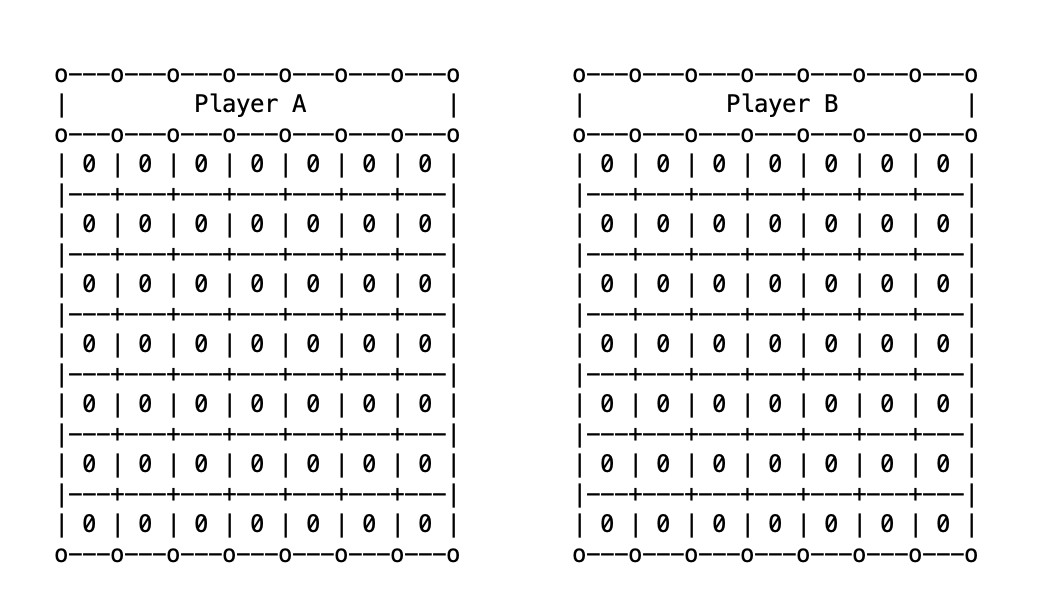
\includegraphics[width=15cm]{graphics/maps.jpg}
        \selectlanguage{english}
        \caption{Initial Maps Interface}
    \end{figure}
    
\end{enumerate}

\newpage

\subsection{Game Logic}
\qquad Let's break down the main functions, focusing on how players take turns placing ships and shooting, including input validation:

\begin{enumerate}
    \item \textbf{Initialization:} \\[6pt]
    \texttt{\$s0}: Grid Size. \\
    \texttt{\$s1}: \textbf{4$\times$1} ships quantity (value: 1). \\
    \texttt{\$s2}: \textbf{3$\times$1} ships quantity (value: 2). \\
    \texttt{\$s3}: \textbf{2$\times$1} ships quantity (value: 3). \\
    \texttt{\$s4}: Player A's map. \\
    \texttt{\$s5}: Player B's map. \\
    \texttt{\$s7}: Player A's turn. \\

    Calls \texttt{game\_menu},  \texttt{rules\_screen}, and  \texttt{print\_maps} to display the menu, rules, and initial maps.

    \item \textbf{Player A Places Ships:} \\[6pt]
    Read Ship Coordinates for Player A:
    \begin{itemize}
        \item Calls \texttt{read\_ship} function with the label \texttt{player\_a\_place\_turn}.
        \item Validates ship placement input using a series of checks (format, size, overlap, etc.).
    \end{itemize}

    \item \textbf{Player B Places Ships:} \\[6pt]
    Read Ship Coordinates for Player B:
    \begin{itemize}
        \item Calls \texttt{read\_ship} function with the label 
        \texttt{player\_b\_place\_turn}.
        \item Similar to Player A, validates ship placement input.
    \end{itemize}

    \item \textbf{Player A Takes a Shot:} \\[6pt]
    Read Shot Coordinates for Player A:
    \begin{itemize}
        \item Calls \texttt{read\_shot} function and displays Player A's label (\texttt{player\_a\_place\_turn}).
        \item Validates shot input using similar checks as ship placement.
    \end{itemize}

    \item \textbf{Player B Takes a Shot:} \\[6pt]
    Read Shot Coordinates for Player B:
    \begin{itemize}
        \item Calls \texttt{read\_shot} function and displays Player B's label (\texttt{player\_b\_place\_turn}).
        \item Validates shot input.
    \end{itemize}

    \item \textbf{Endgame Status Checking:} \\[6pt]
    Check for Win/Loss:
    \begin{itemize}
        \item After each shot, the game checks the status to determine if one of the players has won.
        \item Calls \texttt{endgame\_status\_checking} to check if all ships of the opponent have been hit.
    \end{itemize}

    \item \textbf{Printing Maps:} \\[6pt]
    Print Current State: Calls \texttt{print\_maps} to display the updated maps after ship placements and shots.

    \item \textbf{Exit:} \\[6pt]
    Exiting the Game: The game can be exited at any time by choosing the option to quit (\texttt{[Q]} or \texttt{[q]}).
\end{enumerate}

\newpage

\subsection{Helper Functions}
\begin{enumerate}
    \item \large{\texttt{GAME\_MENU:}}
    
    \qquad The \texttt{game\_menu} function serve the purpose of displaying a menu for the game and allowing the player to start or exit the game based on their input. Let's break down the key components:
    \begin{itemize}
        \item Display Menu Titles:
        \begin{itemize}
            \item The function uses a series of \texttt{la} (\textit{load address}) instructions to load strings (\texttt{title\_0} to \texttt{title\_12}) representing different lines of the menu title.
            \item It prints these titles to the console using the \texttt{SYS\_PRINT\_STRING} system call.
        \end{itemize}
        \item Display Start Prompt: \\
        It prints the string stored at the address \texttt{start} to prompt the player to start the game.
        \item User Input:
        \begin{itemize}
            \item It enters a loop (\texttt{start\_loop}) that prompts the user to input a character.
            \item The input character is stored in \texttt{\$t0}, and an additional read is performed to consume the \texttt{newline ($\backslash$n)} character.
        \end{itemize}
        \item Processing User Input: \\[6pt]
        It checks the input character and proceeds accordingly:
        \begin{itemize}
            \item If the character is \texttt{'y'} or \texttt{'Y'}, it jumps to the label \texttt{game\_menu\_proceed}, suggesting that the player wants to \textit{proceed} with the game.
            \item If the character is \texttt{'n'} or \texttt{'N'}, it jumps to the label \texttt{exit}, indicating that the player wants to \textit{exit} the game.
            \item If the input is anything else, it \textit{continues} the loop (\texttt{start\_loop}) to get a valid input.
        \end{itemize}
        \item End of the Function: \\[6pt]
        The function ends by jumping to the \texttt{jr \$ra} instruction, which returns control to the calling function (\texttt{main}).\\
    \end{itemize}

    \item \large{\texttt{RULES\_SCREEN:}}
    
    \qquad The \texttt{rules\_screen} function serve the purpose of displaying a set of rules to the player and allowing them to choose whether to proceed or return to the game menu based on their input. Let's break down the key components:

    \begin{itemize}
        \item Display Rules:
        \begin{itemize}
            \item The function loads a series of strings (\texttt{rule\_0} to \texttt{rule\_24}) representing different lines of the rules.
            \item It prints these rules to the console using the \texttt{SYS\_PRINT\_STRING} system call.
        \end{itemize}
        \item Display Proceed Prompt: \\[6pt]
        It prints the string stored at the address \texttt{proceed} to prompt the player to either \textit{proceed} or \textit{return} to the game menu.
        \item User Input:
        \begin{itemize}
            \item It enters a loop (\texttt{proceed\_loop}) that prompts the user to input a character.
            \item The input character is stored in \textit{\$t0}, and an additional read is performed to consume the \texttt{newline ($\backslash$n)} character.
        \end{itemize}
        \item Processing User Input: \\[6pt]
        It checks the input character and proceeds accordingly:
        \begin{itemize}
            \item If the character is \texttt{'y'} or \texttt{'Y'}, it jumps to the label \texttt{rules\_screen\_proceed}, suggesting that the player wants to \textit{proceed} with the game.
            \item If the character is \texttt{'n'} or \texttt{'N'}, it jumps to the label \texttt{main}, indicating that the player wants to \textit{return} to the game menu.
            \item If the input is anything else, it \textit{continues} the loop (\texttt{proceed\_loop}) to get a valid input.
        \end{itemize}
        \item End of the Function: \\[6pt]
        The function ends by jumping to the \texttt{jr \$ra} instruction, which returns control to the calling function (\texttt{main}). \\
    \end{itemize}

    \item \large{\texttt{PRINT\_MAPS:}} \\[6pt]
    The \texttt{print\_maps} function have the purpose of printing a game map to the console. It is a textual representation of a grid-based map. Let's break down the key components:

    \begin{itemize}
        \item Print Header: The function starts by printing a header that includes visual separators (\texttt{grid\_bar}) and a label for the player (\texttt{player\_label}).
        \item Initialization: It initializes variables (\texttt{\$t2}, \texttt{\$t3}, and \texttt{\$t0}) that is to be related to map dimensions and loop control.
        \item Print Map Rows: The core functionality involves a loop (\texttt{print\_map}) for printing each row of the map.
        \item Print Grid Elements: Within the row printing loop, the function prints various elements, including grid helpers (\texttt{grid\_helper}), actual values from the map, and visual separators (\texttt{grid\_vert}).
        \item Print Row Transitions: Transitions between different parts of the row are marked with the \texttt{grid\_trans} string.
        \item Loop Control and Row End: The function carefully manages loop control variables (\texttt{\$t1}, \texttt{\$t4}) to control the number of rows printed. It ensures proper termination with the \texttt{print\_row\_loop\_end} label.
        \item Print Footer: A footer is added with \texttt{newline} characters and another visual separator (\texttt{grid\_bar}). \\
    \end{itemize}

    \item \large{\texttt{READ\_SHIP:}} \\[6pt]
    \qquad The \texttt{read\_ship} function is responsible for obtaining and validating user input for placing ships on a game map. The input is expected in the format of ship coordinates, and the function performs various checks to ensure the input adheres to the game's rules.
    \begin{itemize}
        \item Print Prompt: The function starts by printing a prompt (\texttt{prompt\_ship}) to guide the user in entering ship coordinates.
        \item Input Loop: The function enters a loop (\texttt{read\_ship\_loop}) to continuously read and validate ship coordinates until a valid input is provided.
        \item Coordinate Validation:
        \begin{itemize}
            \item It checks for specific user options (\texttt{[R], [r], [Q], [q]}) to either proceed with ship placement or return to the game menu.
            \item Format checking to ensure correct input structure.
            \item Value checking to verify that coordinates are within valid ranges.
            \item Diagonal checking to restrict diagonal ship placement.
        \end{itemize}
        \item Overlap Checking: The function contains a section for checking whether the entered ship coordinates overlap with existing ships on the map.
        \item Placing Ships: Once the input passes all validation checks, the function proceeds to place the ship on the game map.
        \item Error Handling: The function includes various error messages (\texttt{invalid\_format}, \texttt{invalid\_size}, \texttt{invalid\_placement}, \texttt{invalid\_location}) to notify the user of input errors. \\
    \end{itemize}

    \item \large{\texttt{READ\_SHOT:}} \\[6pt]
    \qquad The \texttt{read\_shot} function handles the process of obtaining, validating, and processing user input for shooting at the opponent's game map. It ensures that the entered shot coordinates are valid and performs the corresponding actions based on the game's rules.

    \begin{itemize}
        \item Print Prompt: The function starts by printing a prompt (\texttt{prompt\_shot}) to guide the user in entering shot coordinates.
        \item Player Turn Determination: The function determines the current player's turn based on the value of \texttt{\$s7}. It prompts the appropriate message for the player's turn (\texttt{player\_a\_place\_turn} or \texttt{player\_b\_place\_turn}).
        \item Input Loop: The function enters a loop (\texttt{read\_shot\_loop}) to continuously read, validate, and process shot coordinates until a valid input is provided.
        \item Coordinate Validation:
        \begin{itemize}
            \item It checks for specific user options (\texttt{[R], [r], [Q], [q]}) to either proceed with shooting or return to the game menu.
            Further checks include format checking, ensuring only one space is present, and validating that coordinates are within valid ranges.
        \end{itemize}
        \item Shooting Logic:
        \begin{itemize}
            \item The function distinguishes between Player A's and Player B's turns.
            \item It processes the shot coordinates, checks for hits or misses, updates the opponent's map accordingly, and proceeds to endgame status checking.
        \end{itemize}
        \item Endgame Status Checking: The function checks whether the game has ended by verifying whether all cells on the opponent's map have been hit.
        \item Endgame Messages: It prints messages (\texttt{a\_wins} or \texttt{b\_wins}) based on the winner of the game.
    \end{itemize}

\end{enumerate}
%%%%%%%%%%%%%%%%%%%%%%%%%%%%%%%%%
\section{Conclusion}
\qquad Upon completion of this assignment, students demonstrate proficiency in utilizing the MARS MIPS simulator and applying essential MIPS assembly instructions. The implementation incorporates arithmetic and data transfer instructions, showcasing the students' command over low-level programming concepts. Moreover, the inclusion of conditional branch and unconditional jump instructions reflects a comprehensive understanding of control flow mechanisms in MIPS assembly. \\

\qquad Furthermore, the implementation effectively leverages procedures, emphasizing modular and structured programming practices. The students' ability to navigate the intricacies of the MIPS assembly language is evident throughout the project, culminating in a successful emulation of the Battleship game. This assignment not only serves as a practical application of theoretical knowledge but also showcases the students' aptitude in employing MIPS assembly for real-world programming tasks.
%%%%%%%%%%%%%%%%%%%%%%%%%%%%%%%%%
\begin{thebibliography}{9}
    \bibitem{battleship-wikipedia}
    Wikipedia. (n.d.).
    \textit{Battleship (game).}
    \href{https://en.wikipedia.org/wiki/Battleship (game)}{\texttt{https://en.wikipedia.org/wiki/Battleship (game)}}
    Accessed 2023.
\end{thebibliography}
%%%%%%%%%%%%%%%%%%%%%%%%%%%%%%%%%
\clearpage


\end{document}